\documentclass[../rapport.tex]{subfiles}
\graphicspath{{\subfix{ressources/photos_diagrammes/app2/gui/}}}


\begin{document}


\subsubsection{Application clients}
Cette section décrit les différents interfaces auxquels les employés de l'application auront accès pour gérer leurs clients et leurs produits financier.\\

\begin{enumerate}
    \item \textbf{LoginScene} \\
            \begin{figure}[h!]
                    \centering 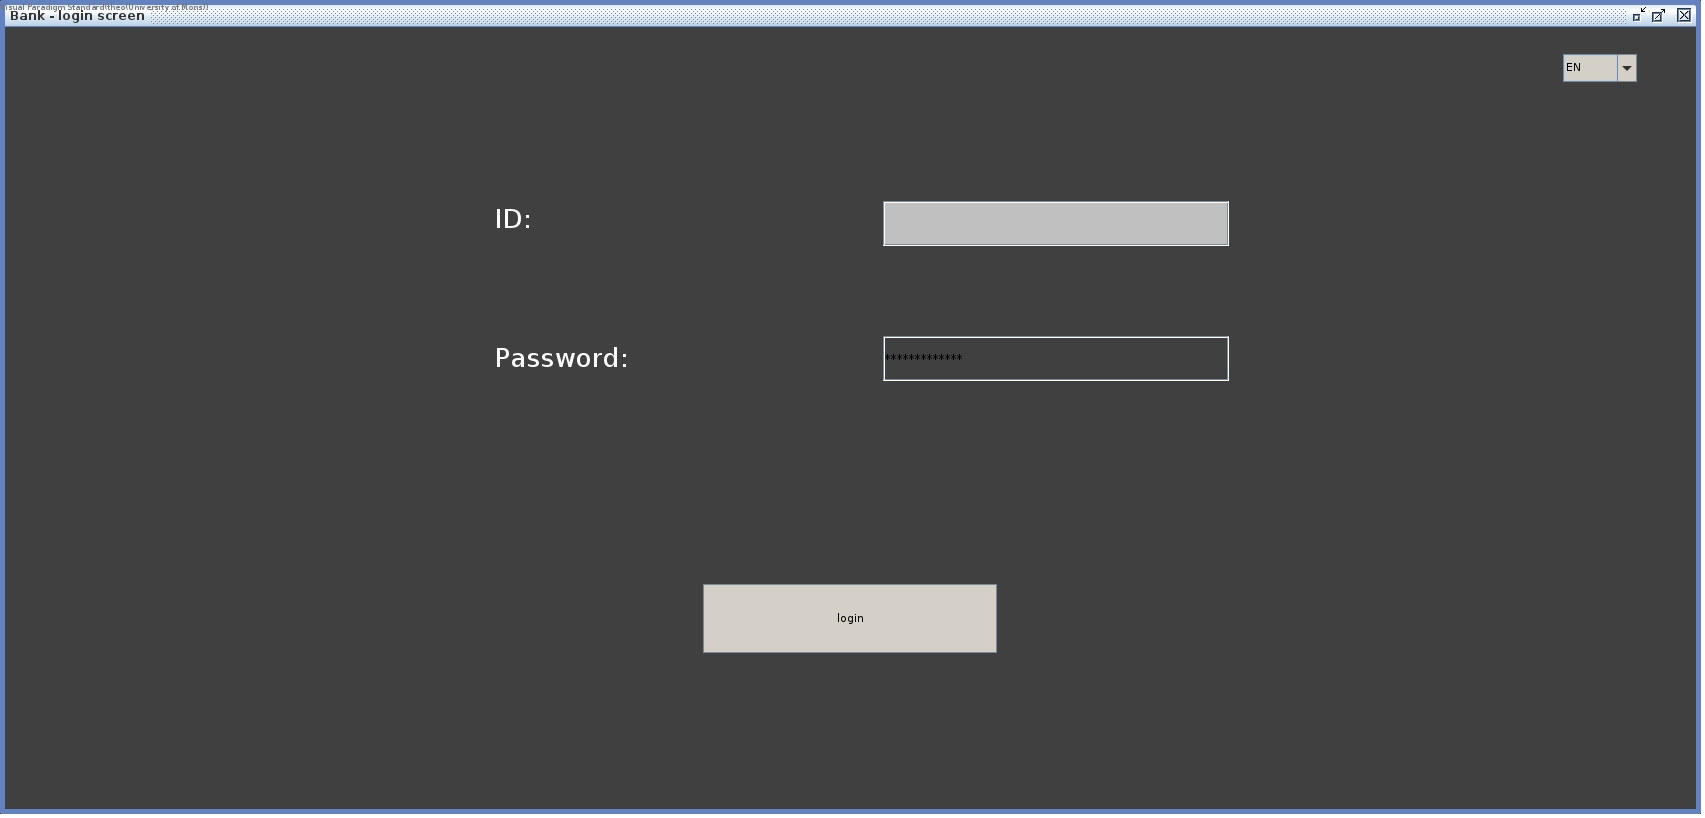
\includegraphics[scale=0.2]{ressources/photos_diagrammes/app2/gui/loginScene.jpg}
                    \caption{Login Scene}
            \end{figure}
            \\
L'écran de connexion est la première interface affichée lors du démarrage de l'application.\\
Cette interface permet à l'employé de l'institution de se connecter via ses identifiants .\\
La langue d'affichage peut également être changée directement depuis le coin supérieur droit.
\newpage
\item \textbf{MainMenuScreen} \\
		\begin{figure}[h!]
				\centering 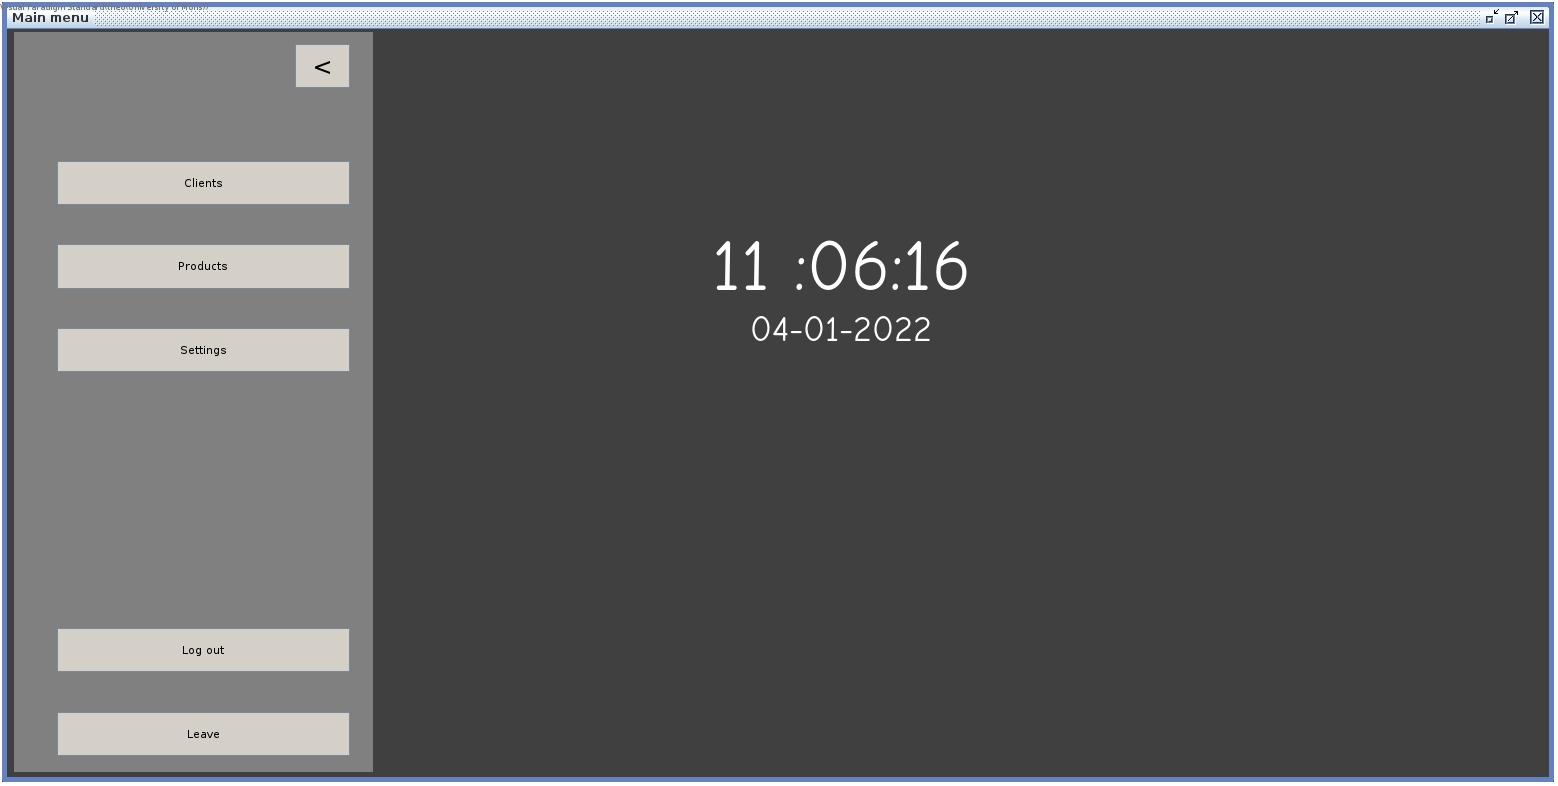
\includegraphics[scale=0.2]{ressources/photos_diagrammes/app2/gui/mainMenuScene.jpg}
				\caption{Main Menu}
		\end{figure}
		\\
Une fois qu'un employé s'est authentifié via le LoginScene, le menu principal lui est affiché. Il permet à l'employé d'accéder au données de l'institution via le menu à 
gauche de l'écran. Il contient un bouton \textit{Clients} qui mène l'employé vers l'écran de listant tout les clients de l'institution.\\
Un bouton \textit{Products} permet à l'employé d'avoir un accès a la liste de tout les produits possédé par des clients. Il pourra y ajouter ou suprimer des produits via cet écran.\\
Le bouton \textit{Settings} mène à l'écran des paramètres de l'app.\\
Le bouton \textit{Log out} permet de se déconnecter (il mène à l'écran de connexion).\\
Et le bouton \textit{Quit} déconnecte l'employé et ferme l'application.
\newpage
\item \textbf{ClientMenuScene} \\
		\begin{figure}[h!]
				\centering 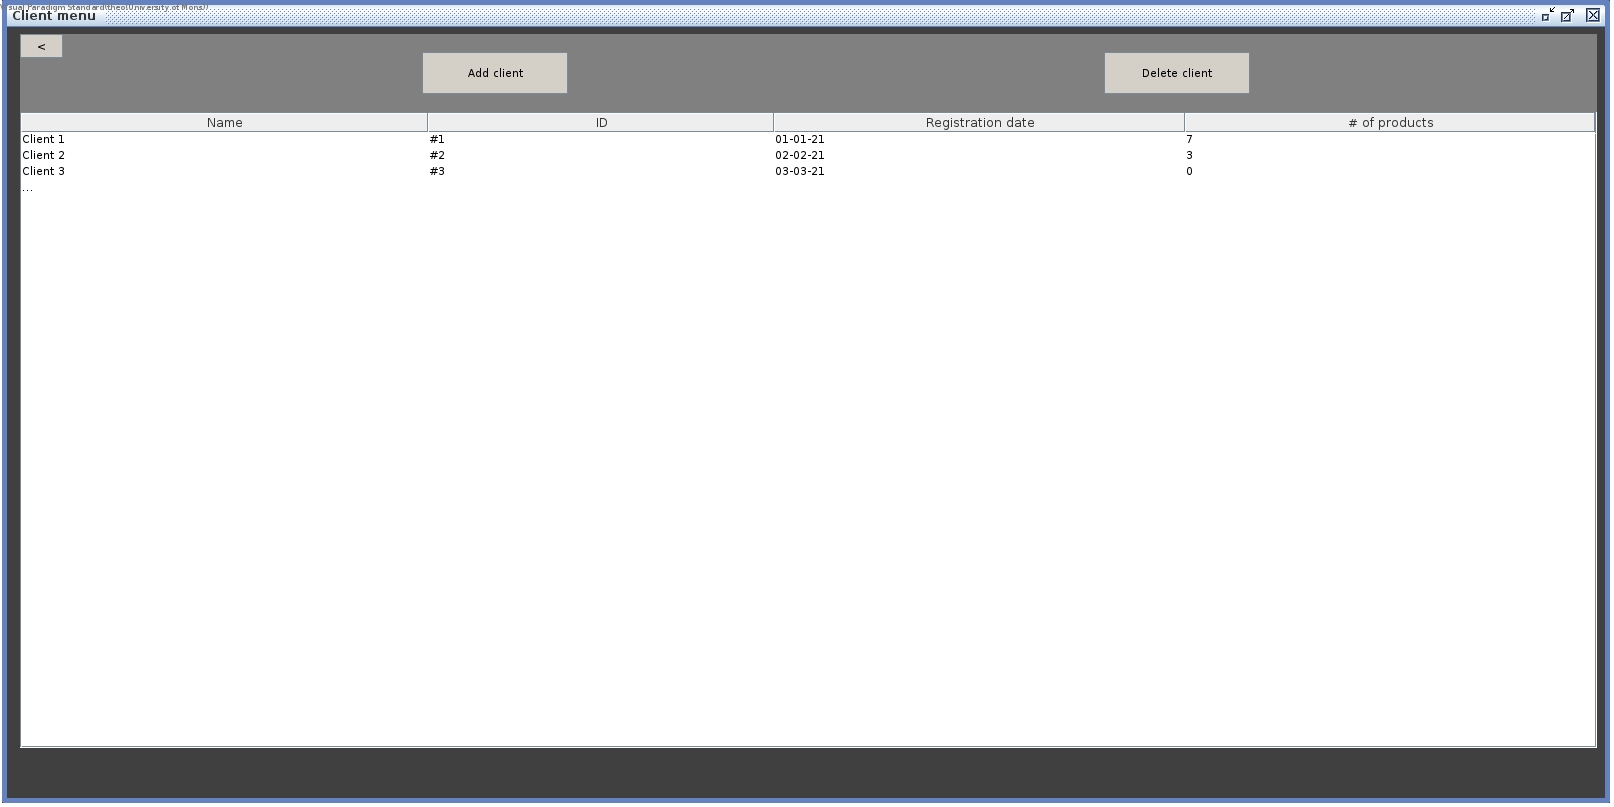
\includegraphics[scale=0.2]{ressources/photos_diagrammes/app2/gui/Clients menu scene.jpg}
				\caption{List of the clients}
		\end{figure}
		\\
L'employé se vois afficher une liste de tout les clients et peux les gerer graces au différents boutons.\\
Le bouton \textit{Add Client} redirige vers le menu d'ajout de clients \textit{addClientMenu}\\
Le bouton \textit{Delete Client} redirige l'employé vers  le menu de supression de client \textit{DeleteClientMenu}\\
Le bouton \textit{back} qui permet de retourner vers \textit{MainMenuScreen}\\
Un clique droit sur un client ouvre le menu supplémentaire \textit{rightClickOnClient}\\
L'employé peux aussi trier les clients en fonctions des différentes caractéristiques listé a l'écran.\\
\newpage
\item \textbf{addClientMenu} \\
		\begin{figure}[h!]
				\centering 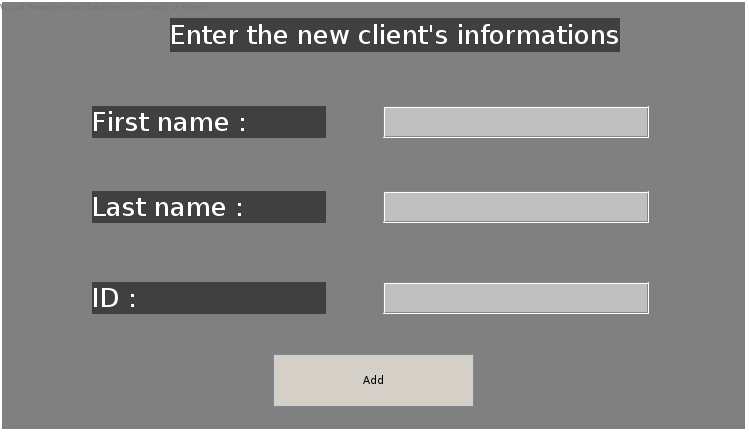
\includegraphics[scale=0.2]{ressources/photos_diagrammes/app2/gui/addClientMenu.jpg}
				\caption{Add client menu}
		\end{figure}
		\\
L'employé peux ajouter un nouveau client en entrant le nom (Last name), le prénom (First name) et le numéro de registre national (ID).\\
Le bouton \textit{Add} permet d'ajouter le client a la liste des clients.\\
\newpage
\item \textbf{delClientMenu} \\
		\begin{figure}[h!]
				\centering 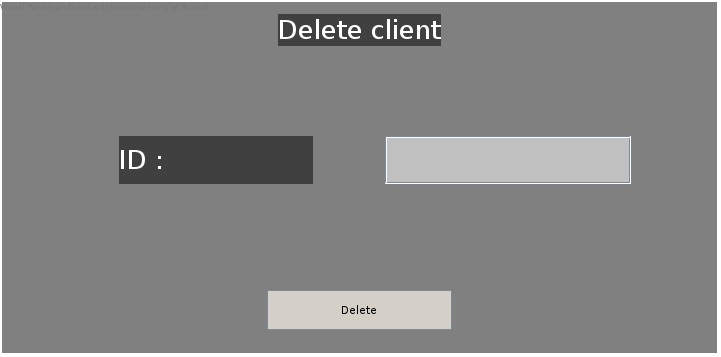
\includegraphics[scale=0.2]{ressources/photos_diagrammes/app2/gui/deleteClientMenu.jpg}
				\caption{Add client menu}
		\end{figure}
		\\
L'employé peux suprimer un client en entrant l'ID (nom\_prenom\_nrRegistreNational) de celui-ci.\\
Le bouton \textit{Delete} permet de supprimer le client de la liste des clients.\\

\newpage
\item \textbf{rightClickOnClient} \\
		\begin{figure}[h!]
				\centering 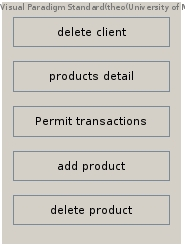
\includegraphics[scale=0.2]{ressources/photos_diagrammes/app2/gui/rightClickOnAClient.jpg}
				\caption{Right click on a client menu}
		\end{figure}
		\\
L'employé peux gerer les clients et leurs produits rapidement grace a ce menu.\\
Le bouton \textit{delete client} va supprimer le client sur le quel l'employé a effectué le clique droit.\\
Le bouton \textit{products detail} va afficher les produits du client sur le quel l'employé a effectué le clique droit.\\
Le bouton \textit{Permit transactions} permettra de rediriger l'employé vers le menu d'autoriser des virement du client sur le quelle clique droit a été effectué.\\
Le bouton \textit{add product} permettra de rediriger l'employé vers le menu d'ajout de produit financier pour le client sur le quel le clique droit a été effectué.\\
Le bouton \textit{delete product} permettra de rediriger l'employé vers le menu de supression de produit financier pour le client sur le quel le clique droit a été effectué.\\
\newpage
\item \textbf{Allow Transaction} \\
		\begin{figure}[h!]
				\centering 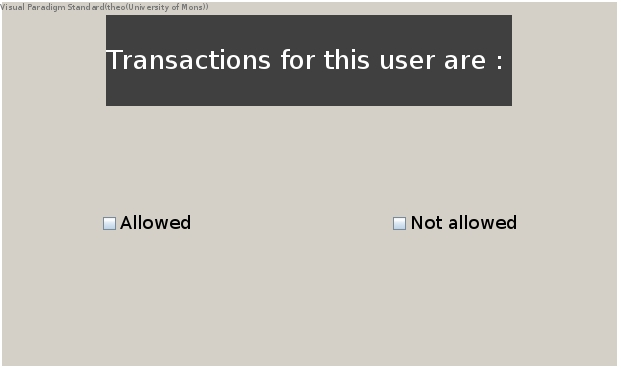
\includegraphics[scale=0.2]{ressources/photos_diagrammes/app2/gui/allowTransactions.jpg}
				\caption{Allow transaction menu}
		\end{figure}
		\\
Ce menu permet a l'employé d'autoriser ou non les transactions du client.\\

\newpage
\item \textbf{ProductMenu Scene} \\
		\begin{figure}[h!]
				\centering 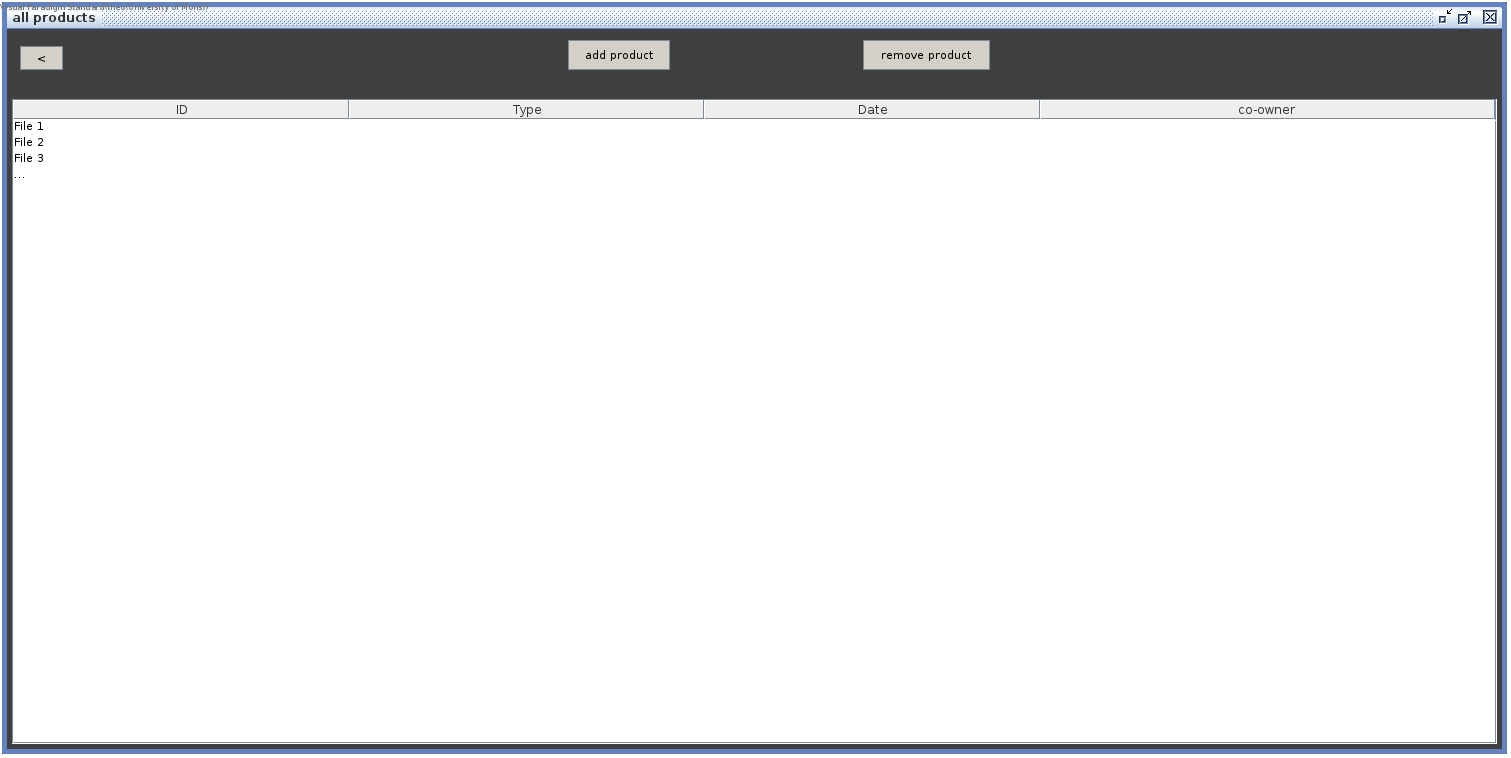
\includegraphics[scale=0.2]{ressources/photos_diagrammes/app2/gui/productsMenuScene.jpg}
				\caption{List of all subscribed to products}
		\end{figure}

Cette scene donne la l'employé la poossibilité de gerer les produits des clients.\\
Un clique sur un produit montrera à l'employé "Clique on a product" avec des informations supplémentaire du produit.\\
Le bouton \textit{add product} permettra de rediriger l'employé vers le menu d'ajout de produit financier pour le client sur le quel le clique droit a été effectué.\\
Le bouton \textit{delete product} permettra de rediriger l'employé vers le menu de supression de produit financier pour le client sur le quel le clique droit a été effectué.\\
Si l'employé éffectue un clique droit sur un produit il accède a un autre menu.\\
\newpage
\item \textbf{add product Scene} \\
		\begin{figure}[h!]
				\centering 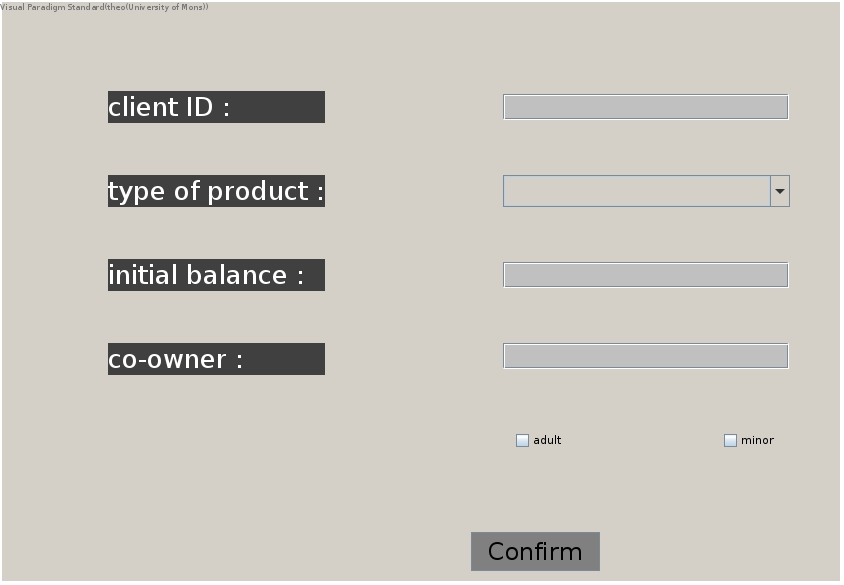
\includegraphics[scale=0.2]{ressources/photos_diagrammes/app2/gui/addFinancialProductMenu.jpg}
				\caption{Add product menu}
		\end{figure}
Ce menu permet a l'employé d'ajouter un nouveau produit financier a un client en y entrant l'ID du client, le sold initial, un co-titulaire éventuelle, si le client est majeur ou pas et de sélectioner le type de produit a ajouter.\\
Le bouton \textit{Confirm} finalise la procédure et ajoute le produit financier au client.\\

\newpage

\item \textbf{delete product Scene} \\
		\begin{figure}[h!]
				\centering 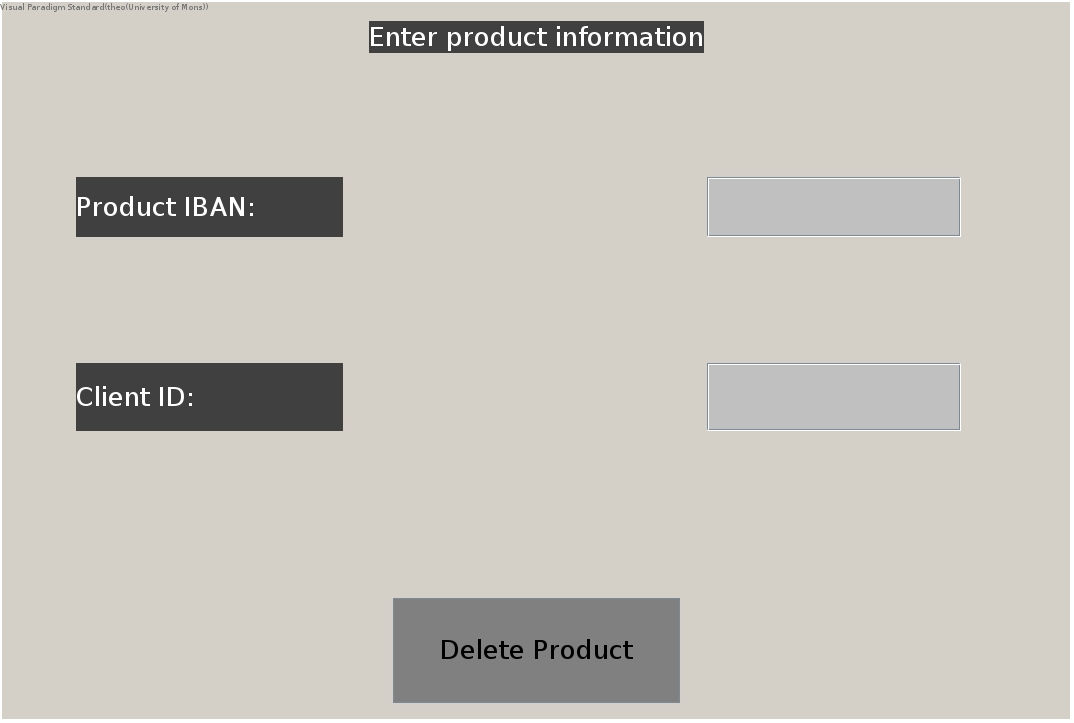
\includegraphics[scale=0.2]{ressources/photos_diagrammes/app2/gui/deleteMenu.jpg}
				\caption{ product menu}
		\end{figure}
Ce menu permet a l'employé de supprimer un produit financier d'un client en y entrant l'ID du client et l'IBAN du produit a supprimer.\\
Le bouton \textit{Confirm} finalise la procédure et supprime le produit financier du client.\\
\newpage
\item \textbf{Client product Scene} \\
		\begin{figure}[h!]
				\centering 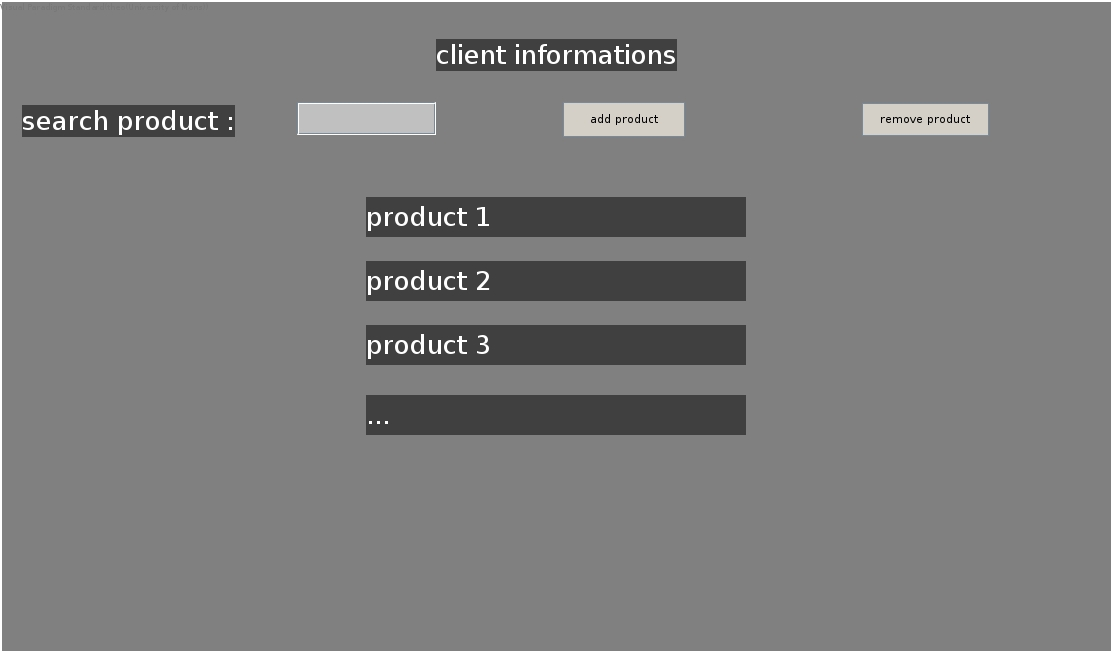
\includegraphics[scale=0.2]{ressources/photos_diagrammes/app2/gui/clientProductMenu.jpg}
				\caption{ Products of a client menu}
		\end{figure}
Cette scene affiche tout les produits financier au quel un client est souscrit et permet à l'employé de les trier en fonction de leurs nom.\\
Le bouton \textit{add product} redirge l'employé vers \textit{add product scene}.\\
Le bouton \textit{remove product redirge} l'employé vers \textit{delete product scene}.\\


\newpage
\item \textbf{Clique on a product} \\
		\begin{figure}[h!]
				\centering 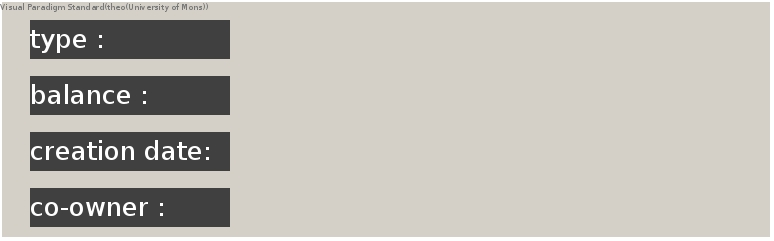
\includegraphics[scale=0.2]{ressources/photos_diagrammes/app2/gui/clickOnAProductInProductMenu.jpg}
				\caption{ Details of a Product }
		\end{figure}
Ce menu affiche des informations supprimentaires sur un produit financier d'un client.\\

\end{enumerate}
\newpage
\end{document}
